\documentclass[conference]{IEEEtran}%,onecolumn
\usepackage[colorlinks,linkcolor=blue,filecolor=blue,citecolor=red,bookmarksnumbered=true]{hyperref}
\usepackage{cite}
\usepackage{graphicx}

\graphicspath{{../reports/}}

\title{Measuring the Global Routing System}

\author{Alexander~Afanasyev %
%,˜\IEEEmembership{Member,˜IEEE,} 
Brent Longstaff, and Neil~Tilley \\ %
\small \{alexander.afanasyev, blongstaff, tilleyns\}@ucla.edu \\ \\
\small Computer Science Department \\
\small University of California, Los Angeles 
} 

\begin{document}

\maketitle

\begin{abstract}
	test
\end{abstract}

% \begin{figure}[htbp]
% 	\centering
% 		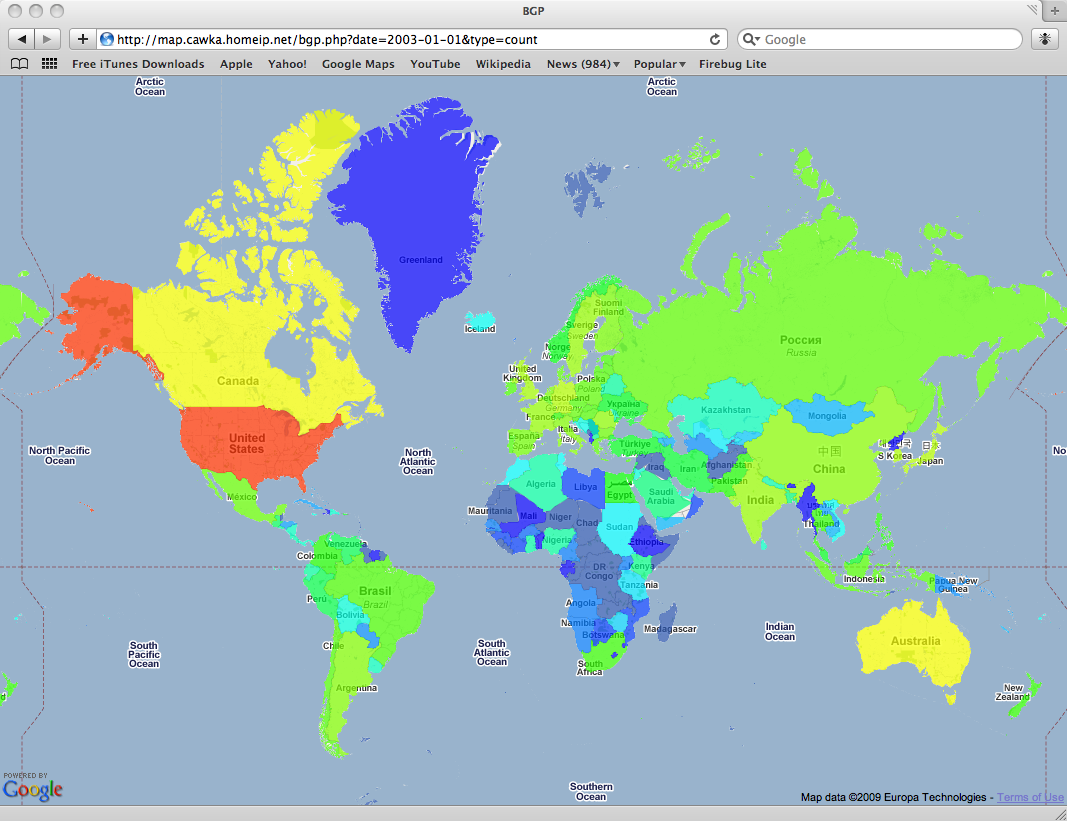
\includegraphics[width=0.5\textwidth]{00_maps/bgp_count_2003}
% 	\caption{caption}
% 	\label{fig:label}
% \end{figure}

\section{Introduction}

BGP is the critical infrastructure for the Internet and interdomain routing.  The routing protocol operates in the junction point where independent networks (an AS, or autonomous system) exchange network traffic through proscribed and announced routes of connectivity.  Because ASes are separate networking and economic entities, BGP must operate balancing essentially two purposes, which are not entirely orthogonal to each other: the limits of efficient networked traffic and the realities of routing policies, which are governed by cost expenses, some issues of politics, network locality, and multihoming preferences.  These have served together, and at times as trade-offs, to add to complexity within BGP and to bring the level of routed Internet traffic -- with its number of policy-constrained routing inefficiencies -- such as is seen at this time.

As originally envisioned, a hierarchical and scalable routing table was to serve as an efficient and streamlined mechanism.  However, not foreseen was how the limited number of IPv4 addresses ($2^{32}$) and the increasing number of allocations to users would lead to fractionalization and finer segmentation of the IP address space.  Fragmentation has effectively flattened portions of the IP address table, rather than preserved the hierarchical IP address-based routing.  Reasons for numerous "special-case" announcements include multihoming demands and Internet customers' implementation of particular traffic engineering to suit any special purposes.  Likewise, single institutions have grown to need more IP addresses than originally allocated and have received additional address blocks that are non-adjacent.  In either case, it has generated a routing table with more entries than a hierarchical structure would have yielded that strictly worked with consolidated blocks.  Correspondingly, the Internet experiences a higher number of transmitted BGP updates to propagate these steadily ongoing changes.  

Several issues impact the growth of the BGP routing table.  First is the challenge of best guessing


% The existing Internet fully relies on the BGP protocol~\cite{Rekhter:1995:RFC1771-BGP} to maintain global connectivity. The key element of the BGP is that each participant (autonomous system, AS) announces its IP prefixes which are propagated to the rest of the ASes by means of the protocol. Although the announced set is generally limited by the address blocks allocated to a particular AS by a Regional Internet Registry (RIR), the AS itself decides the granularity of the announcements. In other words, ASes having only one allocated address block can announce multiple prefixes. The two major reasons for this are traffic engineering and multihoming. The popularity of this prefix splitting can be demonstrated by allocation vs announcement statistics. The number of announced prefixes (160K in 2004~\cite{Meng:2005:IPv4-address} growing 300K in 2009~\cite{::BGP-Reports}) is more than two times the number of allocated IPv4 blocks (65K in 2004, 140K in 2009 respectively). These dynamics cast doubt on global routing scalability.
% 
% As originally envisioned, a hierarchical and scalable routing table was to serve as an efficient and streamlined mechanism. However, not foreseen was how the limited number ($2^{32}$) of IPv4 addresses and alongside the increasing number of allocations to users would lead to fractionalization and finer segmentation of the IP address table. There exist several solutions which attempt to contain the size of the global routing table.  Accompanying the growth of the IP assignments have been aggregation techniques with the intent to gather a group of prefixes under a more general IP prefix. However, Internet customers with particular traffic engineering and multihoming demands have preferred that these guidelines not be implemented. On the other hand, some customers willing to aggregate are not in a position to do so, due to the inability of RIRs to assign a specific requester a contiguous range of IP addresses. Such is the case, for example, with UCLA which has accumulated eight IPv4 address blocks and is forced to announce eight different prefixes (128.97.0.0/16, 131.179.0.0/16, 149.142.0.0/16, 164.67.0.0/16, 169.232.0.0/16, 192.35.210.0/24, 192.35.225.0/24, 192.154.2.0/24). This granular allocation has been one of the major contributors to the growth of the global routing table. An interesting topic to pursue would be to find the average number of allocated blocks assigned to various ASes.
% 
% Meng et al.~\cite{Meng:2005:IPv4-address} reported a number of statistics that will serve as a baseline for our project.  These include 1) the number of allocated blocks and 2) the number of announced prefixes. We propose to conduct more detailed research by country and AS granularity on the ratio and correlation between the number of allocated blocks and the announced prefixes within the BGP routing table. Arguably, any attempt to renumber allocations such that they are less fragmented would reduce both the number of allocations and correspondingly the number of prefixes and size of the BGP table. Our analysis will help to establish an upper bound of the potential BGP routing table reduction if an IPv4 renumbering technique were to be implemented. Additionally, this will justify the necessity of effective IPv6 address assignment and reassignment techniques.

% picture of total # of prefixes
% picture of total # of IP space



The paper is organized as follows.  Section~\ref{sec:data sets} describes the data sets and methodology used in our study.

% Section~\ref{sec:} provides an introduction to the Border Gateway Protocol.    Section 4 presents statistics for IP address allocation and announcement and the BGP table growth.  Section 5 concerns the trends of fragmentation in the BGP routing table.  Section 6 draws a connection between locality and routing table growth, and it shows in which parts of the globe Internet connectivity has been expanding over the last several years.  Section 7 presents data on the longevity and stability of routing table entries.  Related work is discussed in Section 8, followed by the conclusion in Section 9.
\section{Data sets and methodology}
\label{sec:data sets}

some words

\subsection{Data sets}

5 RIRs (ARIN, RIPE NCC, APNIC, LAPNIC, AfriNIC), 5 sources for BGP data (Oregon from RouteViews, Amsterdam, Tokyo, London, Moscow from RIPE NCC),


\subsection{Methodology}

Data is imported to PostgresSQL database for further processing. The total number of collected prefixes is more than 17 000 000.

\section{IP address allocation dynamics}
\label{sec:allocations}



\subsection{Allocated IP block sizes}
\begin{figure}[htbp]
 	\centering
 		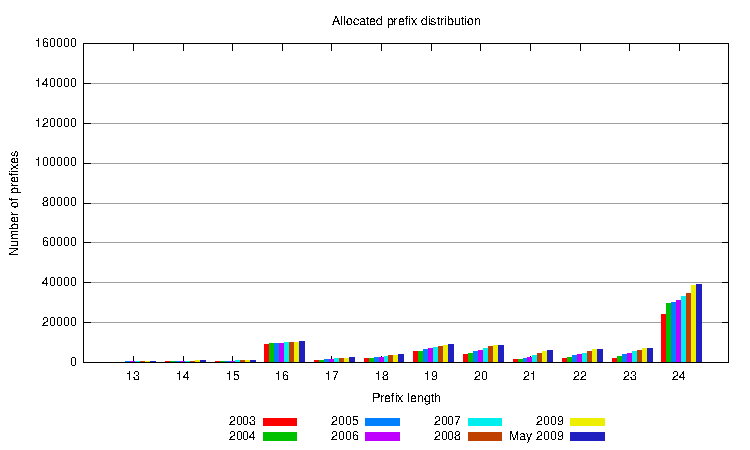
\includegraphics[width=0.5\textwidth]{02_prefixes/02_ip_prefixes_zoom}
	\caption{Allocated prefix distribution}
 	\label{fig:IP allocations}
\end{figure}
The distribution of allocated block sizes has changed over the past six years, as shown in figure \ref{fig:IP allocations}. The number of allocations has increased for every prefix prefix length, but at different rates. In 2003, /24 was the most popular size, as it is today, but there were only about half as many /20 allocations as /19 ones, whereas in 2008 they are about the same. There has been almost no increase in /16 blocks. Throughout the siz-year period, most IP allocations are /24 blocks. The next most popular block size is /16, followed by /19 and /20. The smaller block sizes (/19 and smaller) have had a larger increase in usage than /16, /17, and /18.
\subsection{Yearly distribution of IP allocations}
\begin{figure}[htbp]
 	\centering
 		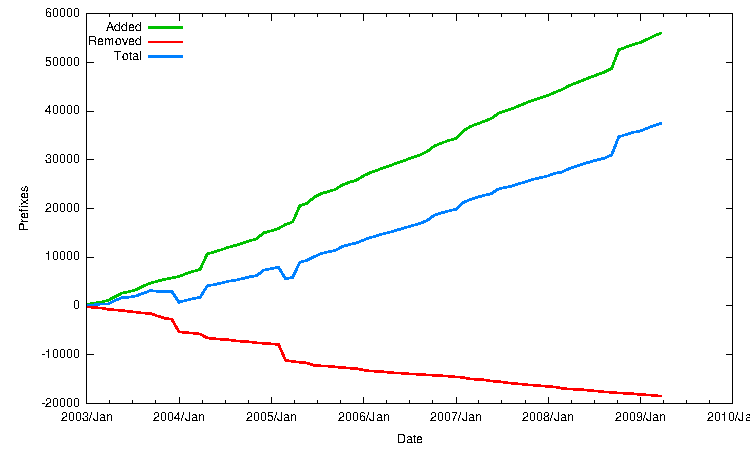
\includegraphics[width=0.5\textwidth]{04_plus_minus/addremoveprefixallocculmulative}
	\caption{Trends in IP prefix allocation}
 	\label{fig:IP allocations new and gone}
\end{figure}
Figure \ref{fig:IP allocations new and gone} shows that the number of allocated IP prefixes has increased by almost 40,000 in the past six years. Some allocations have disappeared, but a larger number of new allocations has outpaced the disappearances.

\subsection{Unaligned allocation}
Unaligned IP allocations are ones whose size is not a power of two. For instance, a block of 1000 addresses could be allocated instead of 1024. The latter could be represented by a single /22 prefix, whereas the former would need a /23, /24, /25, /26, /27, and /29 prefix to express the allocation. Allocations usually have size of a power of two, so a single prefix will suffice. There are not very many unaligned allocations because they are wasteful of BGP table space and have no advantages over aligned ones. Figure \ref{fig:unaligned IP allocations} shows the distribution of such allocations. Most were allocated between 1992 and 1995, although there have been some every year since then. Compared to the size of the entire routing table, these allocations are insignificant, but it is interesting that they exist at all, since RIRs should know better.
\begin{figure}[htbp]
 	\centering
 		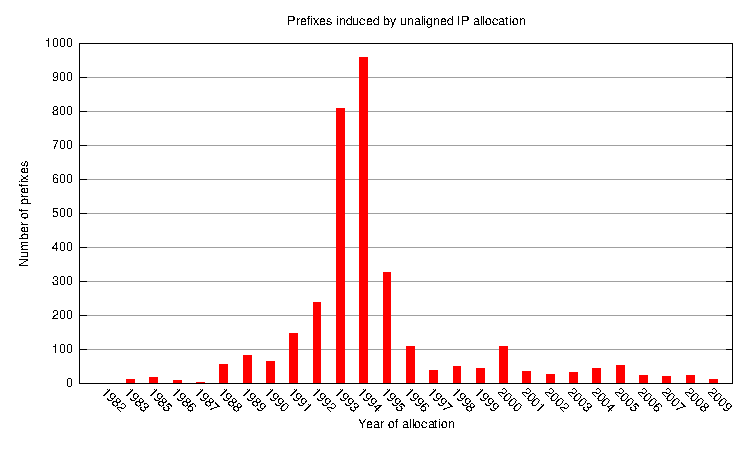
\includegraphics[width=0.5\textwidth]{09_alloc_adhoc/adhoc}
	\caption{Unaligned IP allocations per year}
 	\label{fig:unaligned IP allocations}
\end{figure}
\subsection{Allocation by geographical region}

\subsection{Allocation changes by geographical region}
\begin{figure}[htbp]
 	\centering
 		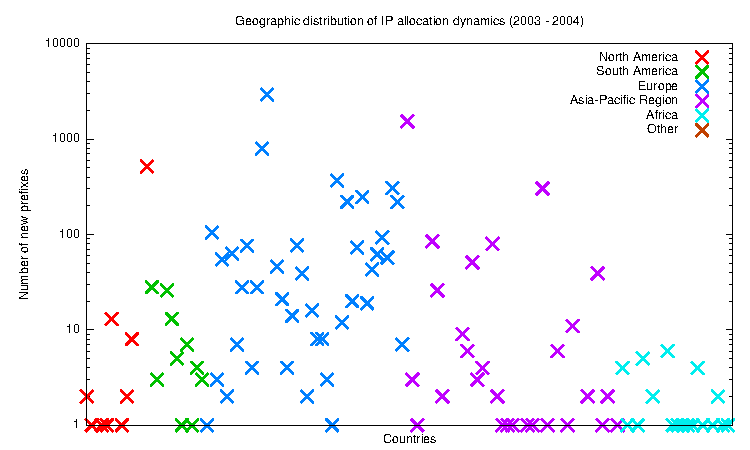
\includegraphics[width=0.5\textwidth]{04_2_plus_minus_countries/plus_minus_2003-01-01}
	\caption{Increase in allocations by region 2003}
 	\label{fig:increase2003}
\end{figure}
\begin{figure}[htbp]
 	\centering
 		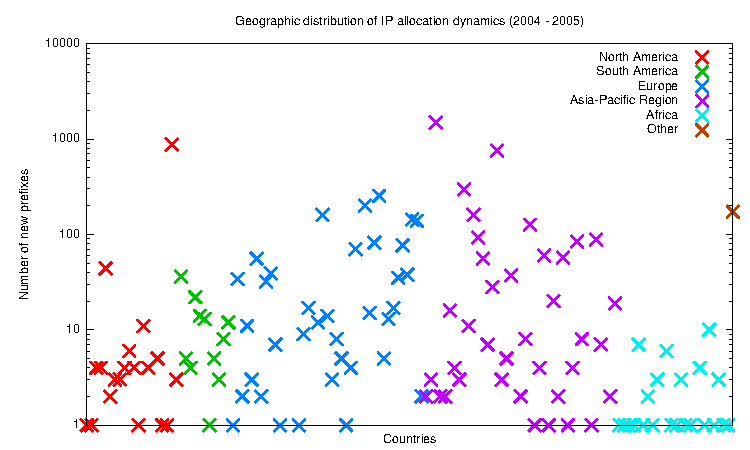
\includegraphics[width=0.5\textwidth]{04_2_plus_minus_countries/plus_minus_2004-01-01}
	\caption{Increase in allocations by region 2004}
 	\label{fig:increase2004}
\end{figure}
\begin{figure}[htbp]
 	\centering
 		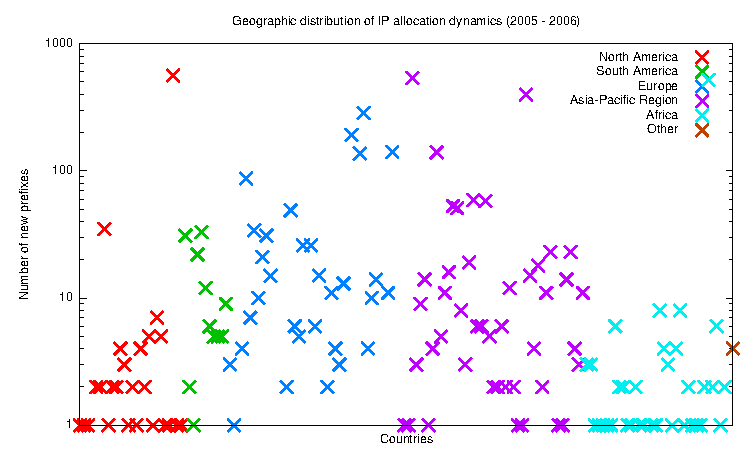
\includegraphics[width=0.5\textwidth]{04_2_plus_minus_countries/plus_minus_2005-01-01}
	\caption{Increase in allocations by region 2005}
 	\label{fig:increase2005}
\end{figure}
\begin{figure}[htbp]
 	\centering
 		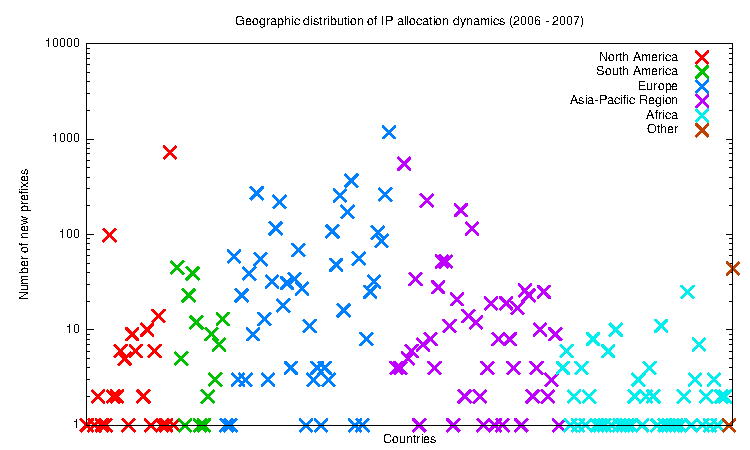
\includegraphics[width=0.5\textwidth]{04_2_plus_minus_countries/plus_minus_2006-01-01}
	\caption{Increase in allocations by region 2006}
 	\label{fig:increase2006}
\end{figure}
\begin{figure}[htbp]
 	\centering
 		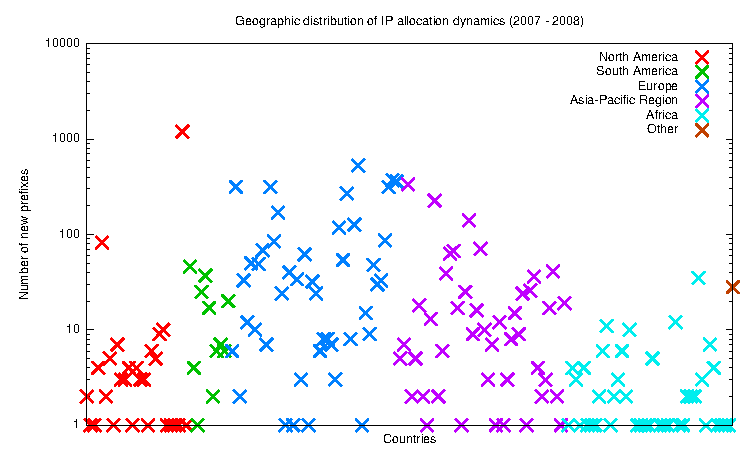
\includegraphics[width=0.5\textwidth]{04_2_plus_minus_countries/plus_minus_2007-01-01}
	\caption{Increase in allocations by region 2007}
 	\label{fig:increase2007}
\end{figure}
\begin{figure}[htbp]
 	\centering
 		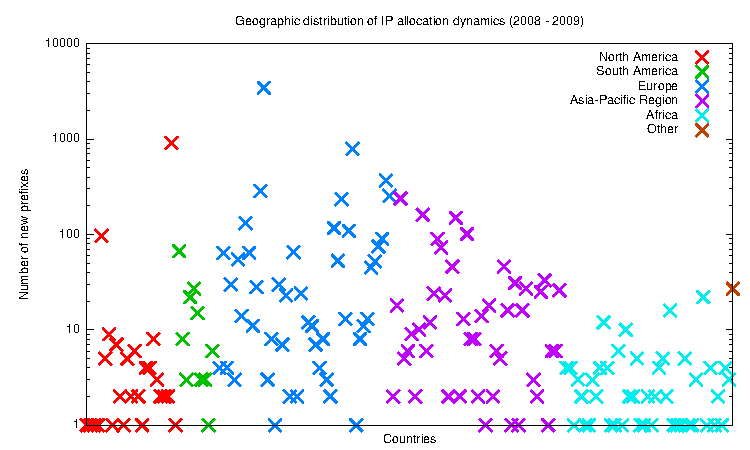
\includegraphics[width=0.5\textwidth]{04_2_plus_minus_countries/plus_minus_2008-01-01}
	\caption{Increase in allocations by region 2008}
 	\label{fig:increase2008}
\end{figure}
As can be seen in figures \ref{fig:increase2003}-\ref{fig:increase2008}, the increase in allocations each years has no clear trend and does not appear to vary in a consistent way. In each country in can vary significantly from one year to the next. The same countries do not allocated more than others every year. 
\section{BGP routing table}
\label{sec:bgp}

In this section we present extensive evaluation of the global routing table
from 2003 to 2009. The first point of our interest is to analyze contribution
of causes to the global routing table growth. That is, we determine how well
ISPs tend to use an allocated address space and how this address space is
subdivided. The second point of interest is to analyze the contents of the BGP
routing table itself. This include an analysis of a level of the overlapping
IP prefix announcements (i.e., how many individual prefixes are also parts of
the bigger prefixes, present in the same routing table). We also show the
stability of the routing table contents. For this purpose, we calculate time
periods during which each individual prefix was visible by the selected BGP
monitor. Finally, we present an evaluation of the BGP routing table entries in
geographical layer, including a tabular and graphical representation of the
BGP entries and numbers of IP addresses, covered by these BGP entries, each
country contributes to the global routing table.

%%%%%%%%%%%%%%%%%%%%%%%%%%%%%%%%%%%%%%%%%%%%%%%%%%%%%%%%%%%%%%%%%%%%%%%%%%%%%
%%%%%%%%%%%%%%%%%%%%%%%%%%%%%%%%%%%%%%%%%%%%%%%%%%%%%%%%%%%%%%%%%%%%%%%%%%%%%
%%%%%%%%%%%%%%%%%%%%%%%%%%%%%%%%%%%%%%%%%%%%%%%%%%%%%%%%%%%%%%%%%%%%%%%%%%%%%
\subsection{Analysis of BGP table growth factors}
%%%%%%%%%%%%%%%%%%%%%%%%%%%%%%%%%%%%%%%%%%%%%%%%%%%%%%%%%%%%%%%%%%%%%%%%%%%%%
%%%%%%%%%%%%%%%%%%%%%%%%%%%%%%%%%%%%%%%%%%%%%%%%%%%%%%%%%%%%%%%%%%%%%%%%%%%%%
%%%%%%%%%%%%%%%%%%%%%%%%%%%%%%%%%%%%%%%%%%%%%%%%%%%%%%%%%%%%%%%%%%%%%%%%%%%%%

The BGP routing table growth is much faster than growth of the number of the
allocated IP blocks (see Figure~\ref{fig:BGP vs RIR}). Currently, the average
number of entries in the global routing table in more than 3 times more than
total number of allocated IP blocks. This increase has dual nature. Firstly,
ISPs tend to subdivide allocated IP blocks into several individual prefixes
and announce them separately. For example, such behavior is very typical for
the transnational providers and providers which lend parts of allocated
address space to its customers, which, in their case, independently announce
lent IP address block. Secondly, various traffic engineering techniques
(traffic balancing, multihoming, etc) create situations when the same address
block is covered by several announced prefixes.

\subsubsection{IP block fragmentation}

Figure~\ref{fig:fragmentation} presents a correlation between allocated IP
blocks and announced IP prefixes. The \emph{matched} curve on the figure
represents IP blocks, which are announced in the exact form as they were
issued by the RIRs. An example of the matched prefix announcement is when an
ISP allocates a block of 1,024 IP addresses (equivalent to /22 block) and then
globally announces this block as a single /22 prefix. As one can see,
currently the number of matched prefixes accounts only 1/6$^{th}$ of the total
number of BGP entries, and this ratio tends to be even smaller in future.

\begin{figure}[htbp]
	\centering
		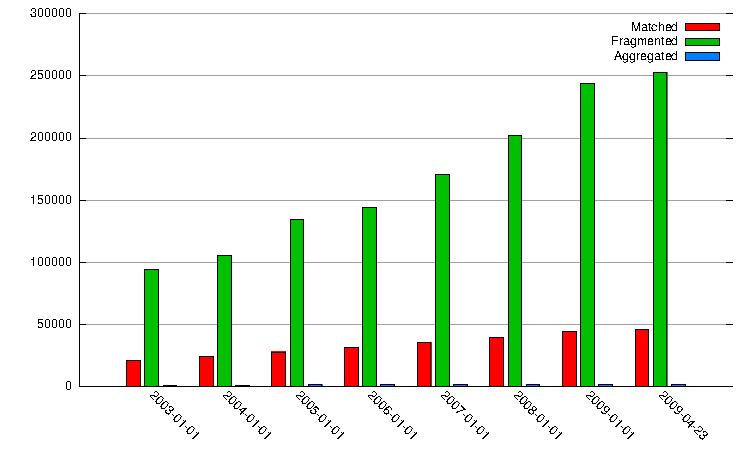
\includegraphics[width=\columnwidth]{05_matched_fragmented/frag-3}
	\caption{Dynamics of matched, fragmented, and aggregated IP prefixes in BGP announcements}
	\label{fig:fragmentation}
\end{figure}

This consideration allows us to make a conclusion that ISPs are not willing to
use allocated address space as is. Instead, they for some reason (e.g.,
geographical dispersion) split up allocated block into a number of sub-blocks
and announce each of the independently. The \emph{fragmented} curve in
Figure~\ref{fig:fragmentation} represents these split up blocks, which
accounts more than 83\% of all entries in global routing table. That is, the
allocated IP block fragmentation is a primary concern for the future BGP
protocol scalability.

The last curve, \emph{aggregated}, represents IP prefix announcements, which
cover several allocated IP blocks. That is, in contrast to the fragmentation,
ISPs, which has several adjacent IP block allocations, are willing to announce
them as a single IP prefix. Unfortunately, the aggregation technique aimed to
reduce hiking number of entries in routing table does not work. In 2003 a
number of aggregated prefixes was 1,400 and this number increased marginally
to nearly 2,000 prefixes in 2009, which is nothing comparing to the total
number of prefixes in the BGP routing table ($\approx$300k).

One surprising conclusion can be made from this analysis. ISPs do not tend to
globally announce the allocated IP space in the original form, no matter of
what size IP block is allocated. This conclusion can serve as a base of
different conclusion concerning future IPv6 deployment. Without a major change
in the BGP protocol, an increase of the allocation IP block size (according to
the current RIRs policy, the minimum allocation IPv6 block is
/32\cite{APNIC:2009:IPv6-Address}) will not help to significantly
reduce the size of global routing table. The only targets for the reduction
are matched IP prefixes (i.e., ISPs which currently use all allocated IP space
as a single block will likely to use a bigger IPv6 space also as a single
block). That is, the upper bound of IP space level optimization is limited by
the number of matched prefixes (less than 17\% of all prefixes).

\subsubsection{Duplicate announcements of IP blocks}

BGP routing table has a consistent trends of containing a large portion of
prefixes, which duplicate each other (Figure~\ref{fig:covered}). In theory,
the IP address coverage duplication in a routing table, where the actual route
is calculated by matching the destination address with the longest available
prefix, is one of the effective ways to reduce a size of the routing table
itself. For example, consider an ISP owning a /8 address block and wanting to
route some /24 block using a different path than the rest of the block. It is
much effective to use a small duplication of address space and only two
entries in routing table, instead of no duplication and 65,536 individual
entries.

\begin{figure}[htbp]
	\centering
		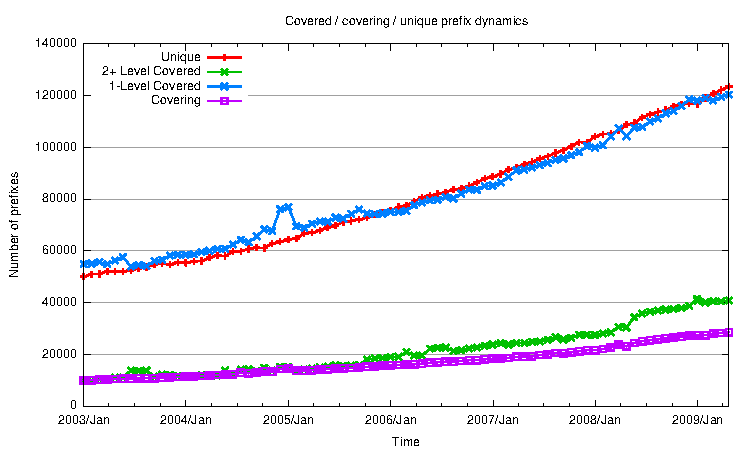
\includegraphics[width=\columnwidth]{06_covered/cover-3}
	\caption{Dynamics of covered, covering, and unique IP prefixes in BGP announcements}
	\label{fig:covered}
\end{figure}

The reality shows that the fundamental IP routing feature of longest prefix
matching is used very extensively. As we can see in Figure~\ref{fig:covered}
(\emph{1 level} curves) number of IP prefixes in BGP table which are covered
by exactly one bigger prefix is nearly the same as number of unique prefixes
(i.e., base prefixes). Moreover, there are substantial amount of prefixes
which has several layers of coverage (several duplication levels, \emph{2+
level} curve).

This high numbers indicate a presence of some additional (besides the
theoretical routing table optimization) incentives for prefix duplication. One
of such factors is a multi-provider connection for end-networks (so called,
multihoming of \emph{stub networks}). According to Oliveira et al.
\cite{Oliveira:2007:Observing-the-evolution}, more than 70\% of all
announcements belongs to multihomed stub networks. In other words, the global
routing table was adopted to serve local or semi-local routing interests of
the majority of customers. It is very unlikely that a customer (a stub
network) connects to providers which are very spaced from each other in the
terms of routing. The conclusion is that if we want to significantly reduce a
size of the BGP routing table, we should find ways to eliminate IP prefix
fragmentation incentives. For example, by providing separate means for
multihoming and traffic engineering tasks.

%%%%%%%%%%%%%%%%%%%%%%%%%%%%%%%%%%%%%%%%%%%%%%%%%%%%%%%%%%%%%%%%%%%%%%%%%%%%%
%%%%%%%%%%%%%%%%%%%%%%%%%%%%%%%%%%%%%%%%%%%%%%%%%%%%%%%%%%%%%%%%%%%%%%%%%%%%%
%%%%%%%%%%%%%%%%%%%%%%%%%%%%%%%%%%%%%%%%%%%%%%%%%%%%%%%%%%%%%%%%%%%%%%%%%%%%%
\subsection{Analysis of the BGP table contents}
%%%%%%%%%%%%%%%%%%%%%%%%%%%%%%%%%%%%%%%%%%%%%%%%%%%%%%%%%%%%%%%%%%%%%%%%%%%%%
%%%%%%%%%%%%%%%%%%%%%%%%%%%%%%%%%%%%%%%%%%%%%%%%%%%%%%%%%%%%%%%%%%%%%%%%%%%%%
%%%%%%%%%%%%%%%%%%%%%%%%%%%%%%%%%%%%%%%%%%%%%%%%%%%%%%%%%%%%%%%%%%%%%%%%%%%%%

Analysis of the BGP routing table contents reveals the current trends and
demands for the IP space. Later in this section we will show an analysis of a
announced prefix size distribution, IP prefix longevity in global BGP
announcements, and geographical distribution of the IP space.

\subsubsection{Lengths of announced IP prefixes}

One of the most critical questions in global routing system is what is the
optimal length of IP prefix to allocate to customers, and what is the optimal
algorithm to select a right prefix to allocate (e.g., how many space should be
reserved after allocated block for the case of the repeated requests from the
same customer). There is a number of solutions to resolve the latter question,
including sequential and bisection allocation schemes, and GAP algorithm
\cite{Wang:2007:Reduce-IP-Address}. The former question is still open.

Figure~\ref{fig:bgp prefix distribution} presents a distribution of the
announced prefix length. The majority of the global routing table entries are
/24-length prefixes (more than 53\% of entries). And during the last 6 years a
number of /24 prefixes practically doubled. At the same time, number of
actually allocated /24 blocks is 4 times smaller (see Figure~\ref{fig:IP
allocations}). This one more time highlights the fact, that a very big number
of stub networks (i.e., relatively small customer networks) are using
announcements of small address blocks to implement multi-provider
connectivity.

\begin{figure}[htbp]
	\centering
		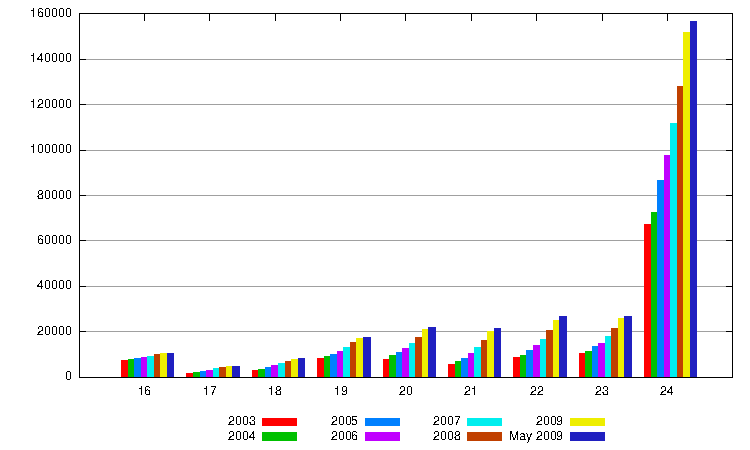
\includegraphics[width=\columnwidth]{02_prefixes/01_bgp_prefixes_zoom}
	\caption{Distribution of announced IP prefix lengths}
	\label{fig:bgp prefix distribution}
\end{figure}

Prefix length of /16 -- /23 has relatively the same level of popularity in the
global routing table, where /17 and /18 has a least popularity. The most
dynamic prefixes from this group are /20 and /21 (growth 2.8 and 3.7 times
respectively), and the least dynamic -- /16 (growth 1.4 times). Another very
interesting observation is for /16 prefix. From the most influential prefixes
(in terms of number of consuming entries in global routing table), the /16
prefix is the only one having a number of global announcements practically
equal to a number of allocations.

The rest of the prefixes has a marginal presence in the global routing table
(total less than 8000 prefixes). This fact shows a small number of entities
having a small (prefixes $<$/16) prefixes and a small number of a tiny
(prefixes $>$/24) customer networks with a multi-provider connectivity.

The results of in this section are additional evidence of the tight
relationship between global routing table growth and IP space fragmentation
and duplication. If we can suppress majority of non-global related
announcements (i.e., bursts of /24 prefixes due to local traffic engineering,
local and semi-local multihoming support, etc), the size of the global routing
table would be significantly reduced.

\subsubsection{Longevity distribution of BGP entries}

Another aspect of the BGP announcement analysis is determining the stability
of the global routing table. In Figure~\ref{fig:bgp ages} presented
distribution of the prefix longevity. The main observation from the graph is
that more than 15\% of the global routing table never changes. On the other
hand, about 15\% (if we compare to the global routing table size in 2009) of
the prefixes were active only for short period of time. A part of these
short-lived prefixes, probably, belongs to spammers who hijack somebody else's
(or nobody's) prefix and announce it for the time to send virtually
untraceable spam messages
\cite{Ramachandran:2006:Understanding-the-network-level}. Some part of the
short-lived prefixes could be explained by the configuration errors. The rest
is, probably, explained by the normal BGP operation where some prefix become
visible only in the case of the primary channel error.

\begin{figure}[htbp]
	\centering
		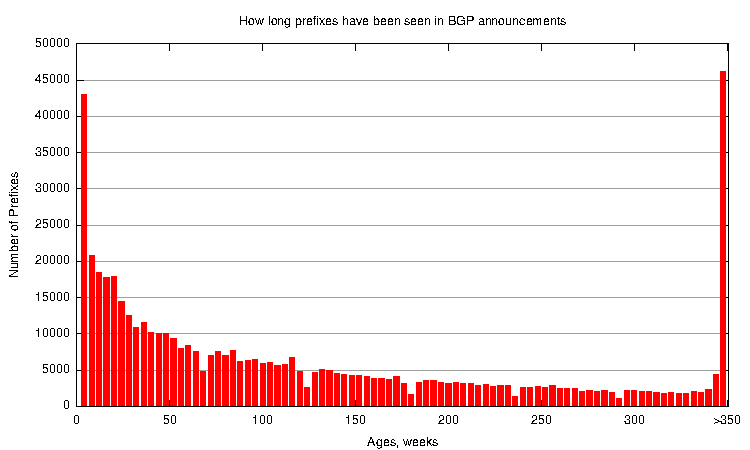
\includegraphics[width=\columnwidth]{08_ages/ages-4}
	\caption{Longevity of prefixes in BGP announcements}
	\label{fig:bgp ages}
\end{figure}

As one can notice from Figure~\ref{fig:bgp ages}, prefix longevity
distribution to some extent is following the exponential distribution
function. That is, besides the fixed number of highly stable routes (15\%), it
is unlikely that some route is visible too long. And in opposite direction,
announced prefixes are likely to have small longevity. This observation shows
the substantial level of the global routing table dynamics.

\subsubsection{BGP announcements by geographical region}
One other direction of our BGP routing system study deals with characteristics
of the allocations and announcements themselves. These are in the areas of
geography and age. Some of the new areas we will examine to monitor where
allocation activity is happening, and for how long a time on average. Thus,
seventh, we will give a year-on-year comparison of prefix allocations and
prefix announcements by major countries, including Russia, Japan, major
countries of Asia, and broad regions such as the European Union, North
America, and Africa.

\begin{figure*}[p]
\centering

%%%%%%%%%%%%%%%%%%%%%%%%%%%%%%%%%%%%%%%%%%%%%%%%%%%%%%%%%%%%%%%%%%
%% BGP counts
%%%%%%%%%%%%%%%%%%%%%%%%%%%%%%%%%%%%%%%%%%%%%%%%%%%%%%%%%%%%%%%%%%
\begin{minipage}[b]{0.48\textwidth}
% \begin{figure}[p]
	\centering
		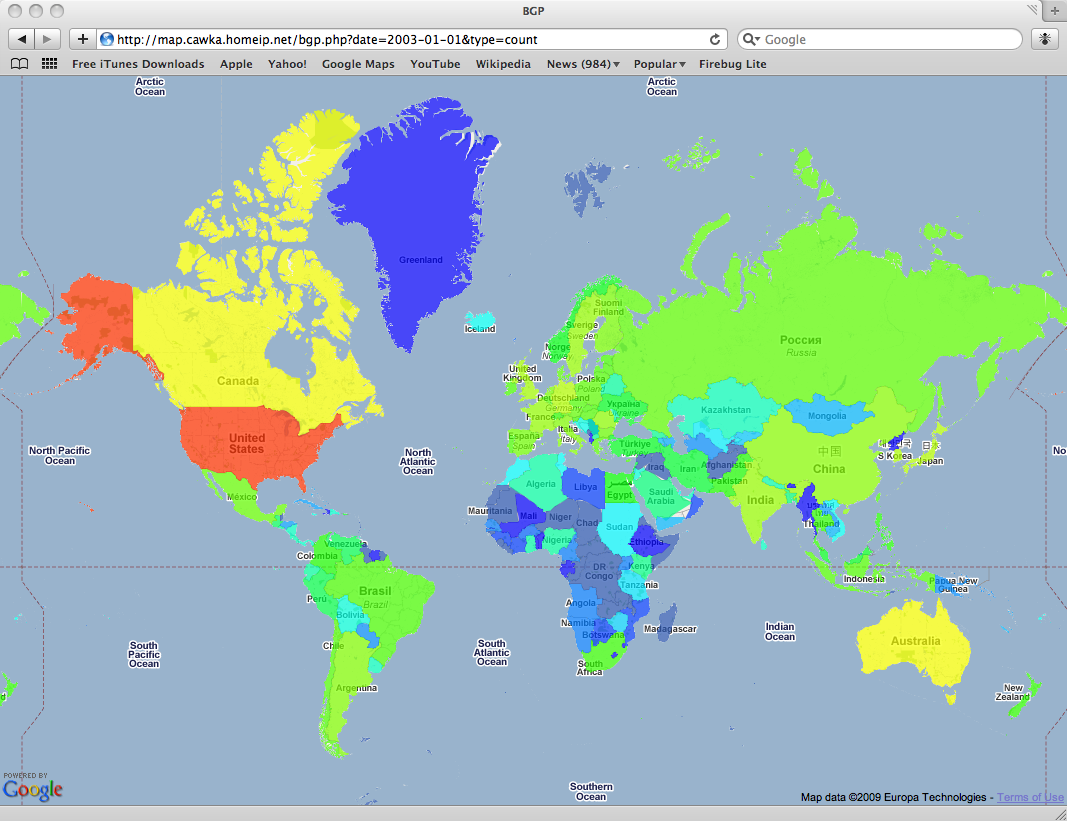
\includegraphics[trim=0 17px 0px 76px,clip=true,width=\columnwidth]{00_maps/bgp_count_2003}%
		\hspace{-0.98\columnwidth}%
		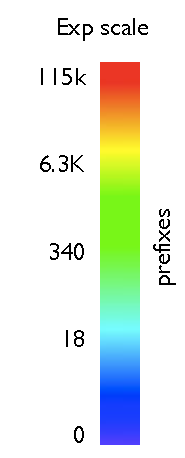
\includegraphics[width=1cm]{scale_bgp_count}\hspace{-1cm}%
		\hspace{0.98\columnwidth}
	\caption{Geographical distribution of number of announced prefixes on \textbf{January 1, 2003}}
	\label{fig:bgp prefixes 2003}
% \end{figure}
\end{minipage}%
%
\quad
%
\begin{minipage}[b]{0.48\textwidth}
% \begin{figure}[p]
	\centering
		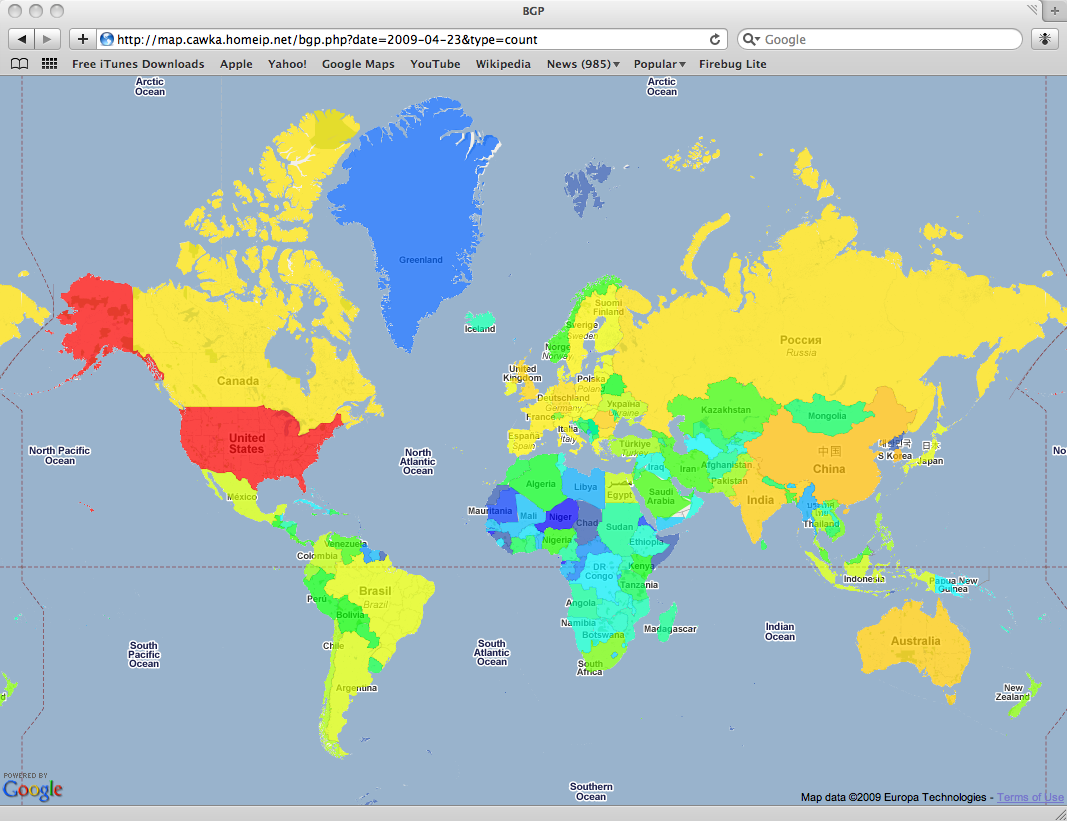
\includegraphics[trim=0 17px 0px 76px,clip=true,width=\columnwidth]{00_maps/bgp_count_2009_2}%
		\hspace{-0.98\columnwidth}%
		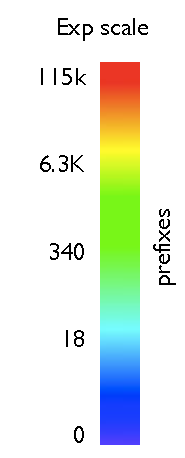
\includegraphics[width=1cm]{scale_bgp_count}\hspace{-1cm}%
		\hspace{0.98\columnwidth}
	\caption{Geographical distribution of number of announced prefixes on \textbf{April 23, 2009}}
	\label{fig:bgp prefixes 2009}
% \end{figure}
\end{minipage}

\vspace{0.5cm}

%%%%%%%%%%%%%%%%%%%%%%%%%%%%%%%%%%%%%%%%%%%%%%%%%%%%%%%%%%%%%%%%%%
%% BGP sizes
%%%%%%%%%%%%%%%%%%%%%%%%%%%%%%%%%%%%%%%%%%%%%%%%%%%%%%%%%%%%%%%%%%
\begin{minipage}[b]{0.48\textwidth}
% \begin{figure}[p]
	\centering
		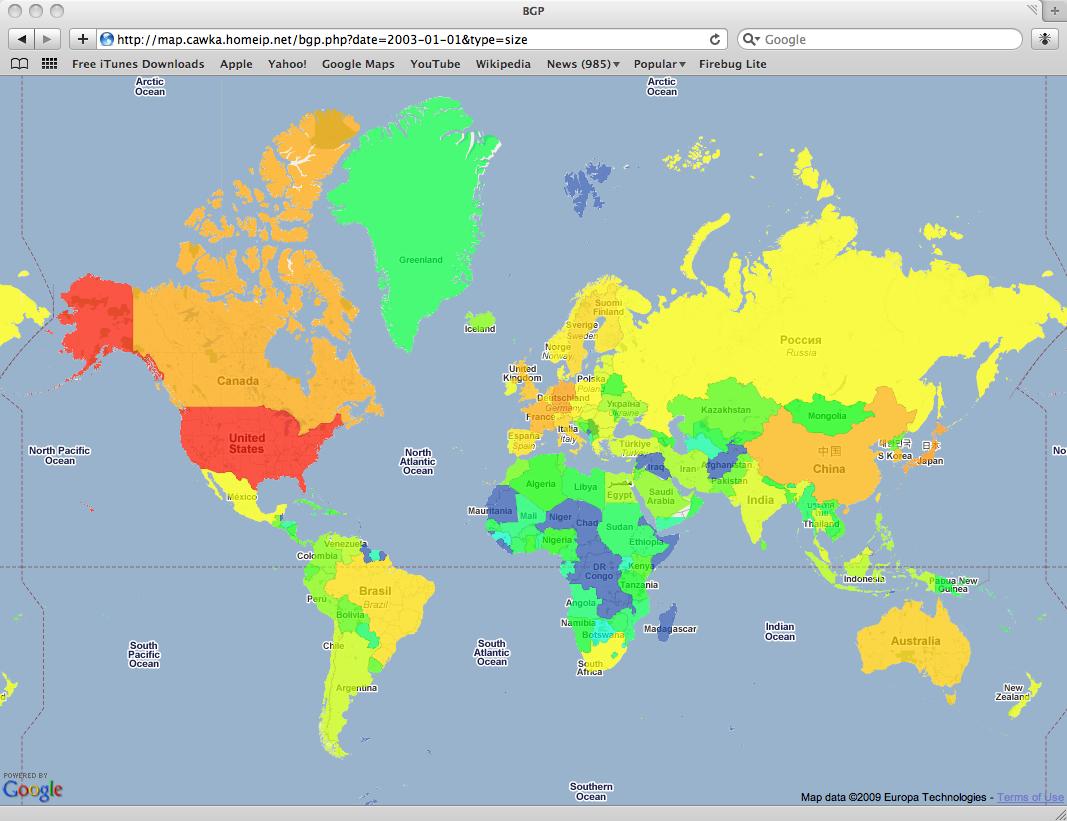
\includegraphics[trim=0 17px 0px 76px,clip=true,width=\columnwidth]{00_maps/bgp_size_2003}%
		\hspace{-0.98\columnwidth}%
		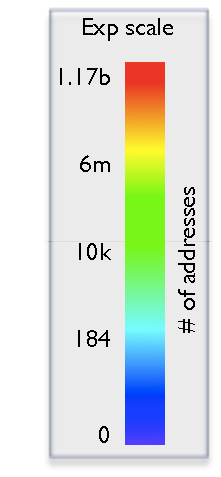
\includegraphics[width=1cm]{scale_bgp_size}\hspace{-1cm}%
		\hspace{0.98\columnwidth}
	\caption{Geographical distribution of announced IP space on \textbf{January 1, 2003}}
	\label{fig:bgp ip space 2003}
% \end{figure}
\end{minipage}%
%
\quad
%
\begin{minipage}[b]{0.48\textwidth}
% \begin{figure}[p]
	\centering
		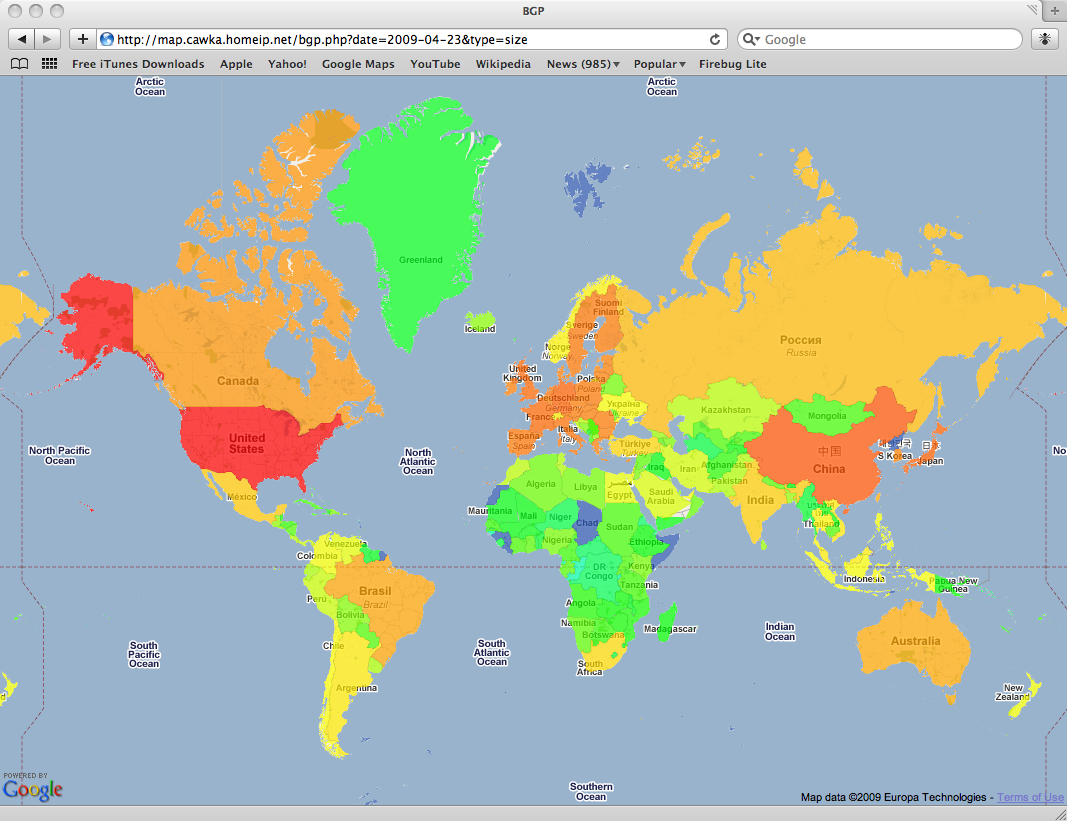
\includegraphics[trim=0 17px 0px 76px,clip=true,width=\columnwidth]{00_maps/bgp_size_2009_2}%
		\hspace{-0.98\columnwidth}%
		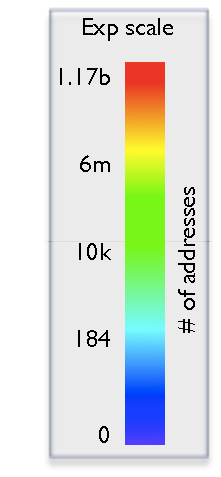
\includegraphics[width=1cm]{scale_bgp_size}\hspace{-1cm}%
		\hspace{0.98\columnwidth}
	\caption{Geographical distribution of announced IP space on \textbf{April 23, 2009}}
	\label{fig:bgp ip space 2009}
% \end{figure}
\end{minipage}

\vspace{0.5cm}

%%%%%%%%%%%%%%%%%%%%%%%%%%%%%%%%%%%%%%%%%%%%%%%%%%%%%%%%%%%%%%%%%%
%% Asia region
%%%%%%%%%%%%%%%%%%%%%%%%%%%%%%%%%%%%%%%%%%%%%%%%%%%%%%%%%%%%%%%%%%
\begin{minipage}[b]{0.48\textwidth}
% \begin{figure}[p]
	\centering
		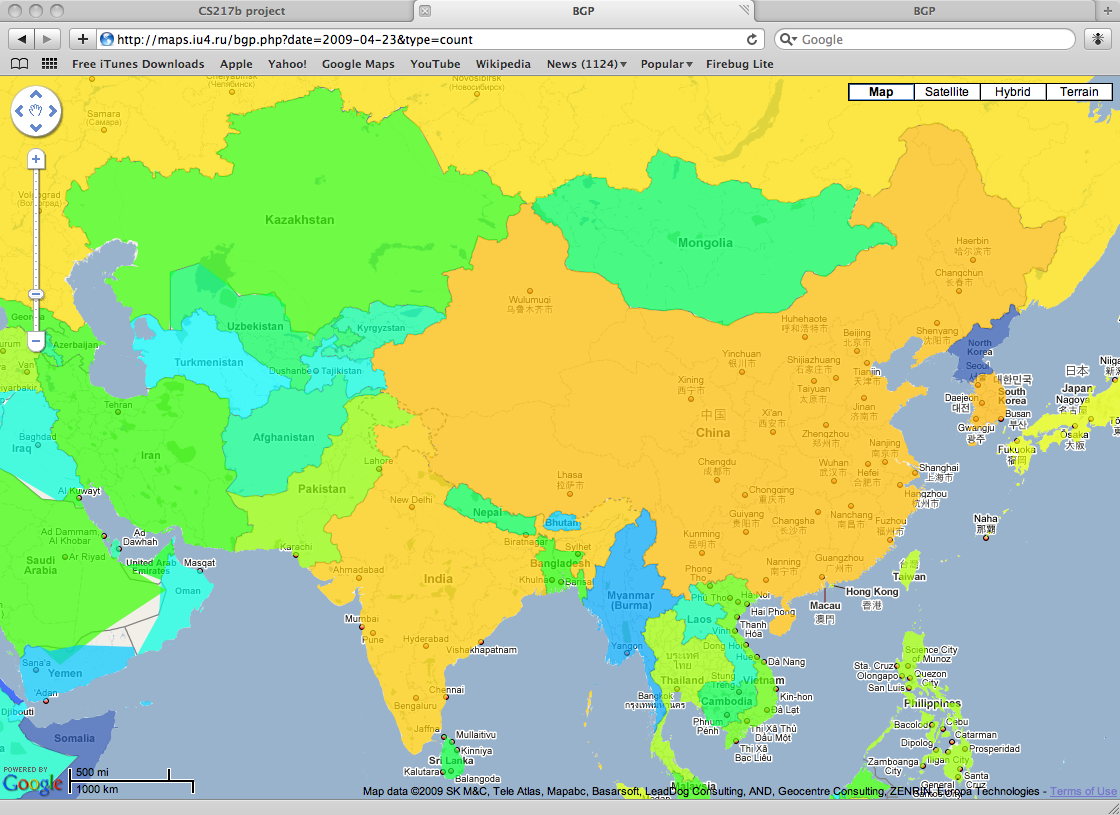
\includegraphics[trim=0 17px 0px 76px,clip=true,width=\columnwidth]{00_maps/asia_2009_prefixes}%
		\hspace{-0.98\columnwidth}%
		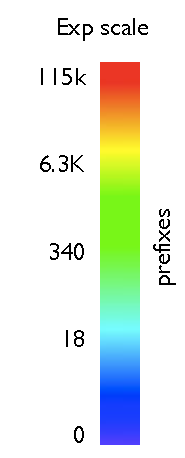
\includegraphics[width=1cm]{scale_bgp_count}\hspace{-1cm}%
		\hspace{0.98\columnwidth}
	\caption{Geographical distribution of number of announced prefixes in Asian region on \textbf{April 23, 2009}}
	\label{fig:bgp prefixes asia 2009}
% \end{figure}
\end{minipage}%
%
\quad
%
\begin{minipage}[b]{0.48\textwidth}
% \begin{figure}[p]
	\centering
		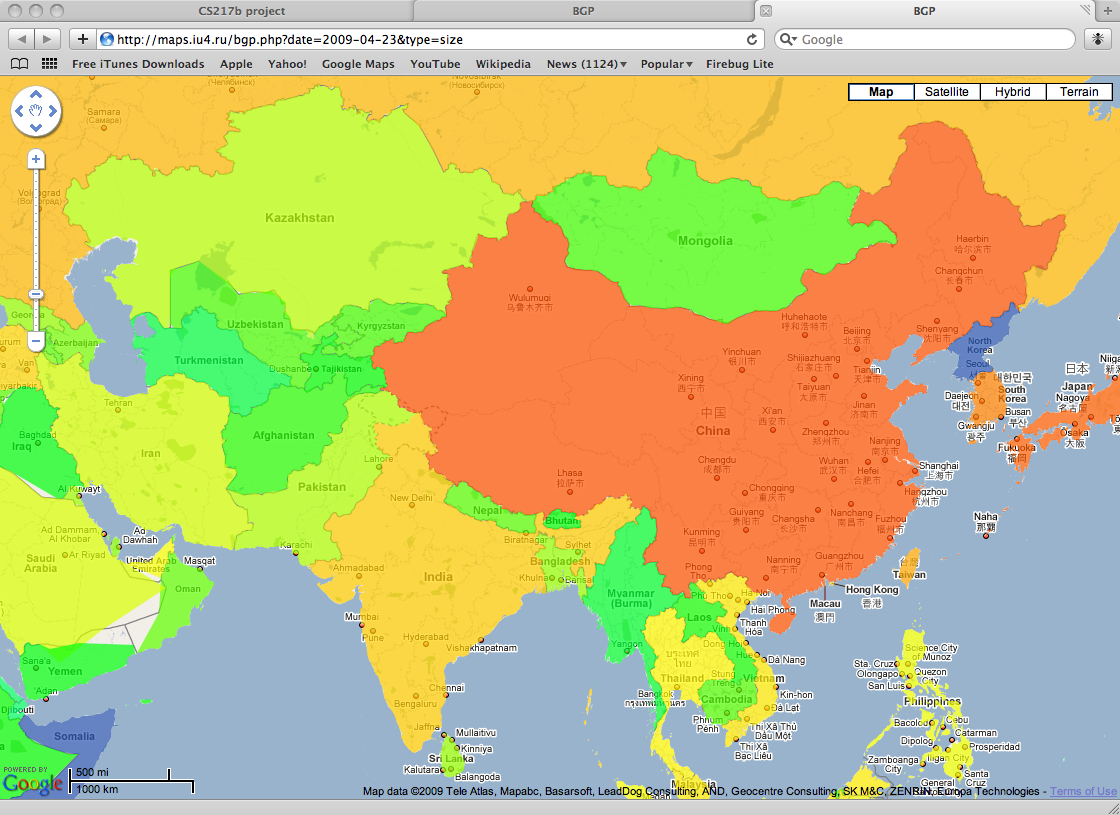
\includegraphics[trim=0 17px 0px 76px,clip=true,width=\columnwidth]{00_maps/asia_2009_space}%
		\hspace{-0.98\columnwidth}%
		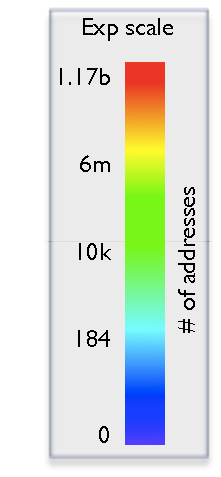
\includegraphics[width=1cm]{scale_bgp_size}\hspace{-1cm}%
		\hspace{0.98\columnwidth}
	\caption{Geographical distribution of announced IP space in Asian region on \textbf{April 23, 2009}}
	\label{fig:bgp ip space asia 2009}
% \end{figure}
\end{minipage}

\end{figure*}

% \clearpage


\begin{table*}[p]
%%%%%%%%%%%%%%%%%%%%%%%%%%%%%%%%%%%%%%%%%%%%%%%%%%%%%%%%%%%%%%%%%%%%%%%%%%%%%%%%
%% TOP announced prefixes
%%%%%%%%%%%%%%%%%%%%%%%%%%%%%%%%%%%%%%%%%%%%%%%%%%%%%%%%%%%%%%%%%%%%%%%%%%%%%%%%
\begin{minipage}[t]{0.48\textwidth}
% \begin{table}[p]
	\begin{center}
	\caption{Top 25 countries with the most number of announced prefixes in BGP table on \textbf{January 1, 2003}}
	\label{tab:top25 bgp prefixes 2003}
	\begin{tabular}{|l||l|r|r|} %\hline
		\hline
		&      \bf Country		&    Prefixes   &       IP space 		\tabularnewline \hline 
1       &       US      		&       65849   &       759,792,816     \tabularnewline %\hline
2       &       \emph{Unknown}	&       6258    &       68,926,314      \tabularnewline %\hline
3       &       Australia       &       5762    &       17,822,159      \tabularnewline %\hline
4       &       Canada  		&       5612    &       38,912,924      \tabularnewline %\hline
5       &       Japan   		&       2633    &       58,905,280      \tabularnewline %\hline
6       &       South Korea     &       2441    &       27,334,687      \tabularnewline %\hline
7       &       Germany			&       1934    &       46,556,556      \tabularnewline %\hline
8       &       India  			&       1931    &       2,943,040       \tabularnewline %\hline
9       &       UK     			&       1873    &       32,626,649      \tabularnewline %\hline
10      &       China  			&       1615    &       28,522,130      \tabularnewline %\hline
11      &       Argentina       &       1477    &       2,017,448       \tabularnewline %\hline
12      &       Hong Kong       &       1261    &       5,621,473       \tabularnewline %\hline
13      &       Sweden  		&       1198    &       11,280,533      \tabularnewline %\hline
14      &       France  		&       1148    &       31,320,040      \tabularnewline %\hline
15      &       Mexico  		&       1059    &       5,275,520       \tabularnewline %\hline
16      &       Romania 		&       994     &       667,136 		\tabularnewline %\hline
17      &       Russia  		&       972     &       5,911,712       \tabularnewline %\hline
18      &       Chile   		&       834     &       2,098,161       \tabularnewline %\hline
19      &       Indonesia       &       830     &       1,170,560       \tabularnewline %\hline
20      &       Italy   		&       791     &       13,324,288      \tabularnewline %\hline
21      &       Brazil  		&       760     &       11,580,416      \tabularnewline %\hline
22      &       Taiwan  		&       708     &       13,448,168      \tabularnewline %\hline
23      &       Netherlands     &       689     &       19,939,341      \tabularnewline %\hline
24      &       European Union  &       687     &       2,707,383       \tabularnewline %\hline
25      &       Finland 		&       630     &       7,307,018       \tabularnewline %\hline
% 26      &       South Africa    &       618     &       5,762,180       \tabularnewline %\hline
% 27      &       New Zealand     &       566     &       3,828,620       \tabularnewline %\hline
% 28      &       Switzerland     &       560     &       7,937,424       \tabularnewline %\hline
% 29      &       Thailand        &       559     &       1,877,060       \tabularnewline %\hline
% 30      &       Spain   		&       511     &       8,921,568       \tabularnewline %\hline
	\hline
	\end{tabular}
	\end{center}
% \end{table}
\end{minipage}
%
\quad
%
\begin{minipage}[t]{0.48\textwidth}
% \begin{table}[p]
	\begin{center}
	\caption{Top 25 countries with the most number of announced prefixes in BGP table on \textbf{April 23, 2009}}
	\label{tab:top25 bgp prefixes 2009}
	\begin{tabular}{|l||l|r|r|r|}
		\hline
		&      \bf Country		& \bf Prefixes  &       \bf IP space 	& \bf Change$^{*}$ 	\tabularnewline \hline 
1       &       US      		&       115780  &       1,170,481,177   & 1.54			\tabularnewline %\hline
2       &       South Korea     &       14308   &       84,553,300      & 3.09			\tabularnewline %\hline
3       &       China  			&       13188   &       223,990,021     & 7.85			\tabularnewline %\hline
4       &       Australia       &       11329   &       37,818,072      & 2.12			\tabularnewline %\hline
5       &       India   		&       11022   &       17,575,040      & 5.97			\tabularnewline %\hline
6       &       Russia  		&       8650    &       26,664,224      & 4.51			\tabularnewline %\hline
7       &       Canada  		&       8328    &       57,471,348      & 1.48			\tabularnewline %\hline
8       &       Romania 		&       5729    &       7,348,881       & 11.02			\tabularnewline %\hline
9       &       UK      		&       5269    &       63,871,082      & 1.96			\tabularnewline %\hline
10      &       European Union  &       4937    &       87,825,582      & 32.44			\tabularnewline %\hline
11      &       Japan   		&       4674    &       173,789,965     & 2.95			\tabularnewline %\hline
12      &       Brazil  		&       4643    &       40,429,504      & 3.49			\tabularnewline %\hline
13      &       Argentina       &       4142    &       9,721,411       & 4.82			\tabularnewline %\hline
14      &       Germany 		&       4035    &       84,904,642      & 1.82			\tabularnewline %\hline
15      &       Mexico  		&       3648    &       19,583,832      & 3.71			\tabularnewline %\hline
16      &       Indonesia       &       3562    &       5,248,256       & 4.48			\tabularnewline %\hline
17      &       Hong Kong       &       3459    &       14,764,300      & 2.63			\tabularnewline %\hline
18      &       \emph{Unknown}	&       3393    &       37,265,411      & 				\tabularnewline %\hline
19      &       Bulgaria        &       3325    &       4,439,040       & 7.72			\tabularnewline %\hline
20      &       Colombia        &       3029    &       4,901,340       & 11.86			\tabularnewline %\hline
21      &       Ukraine 		&       3028    &       5,547,136       & 7.67			\tabularnewline %\hline
22      &       Egypt  			&       2992    &       3,854,848       & 4.60			\tabularnewline %\hline
23      &       France 			&       2511    &       61,070,996      & 1.95			\tabularnewline %\hline
24      &       Taiwan 			&       2511    &       36,623,744      & 2.72			\tabularnewline %\hline
25      &       Chile  			&       2375    &       6,101,376       & 2.91			\tabularnewline %\hline
% 26      &       Poland 			&       2341    &       15,122,881      & 4.06			\tabularnewline %\hline
% 27      &       Thailand        &       2039    &       7,210,800       & 3.84			\tabularnewline %\hline
% 28      &       Spain   		&       1989    &       25,315,136      & 2.84			\tabularnewline %\hline
% 29      &       Sweden  		&       1942    &       18,532,345      & 1.64			\tabularnewline %\hline
% 30      &       Turkey  		&       1940    &       14,309,632      & 6.41			\tabularnewline %\hline
	\hline
	\end{tabular}
	\end{center}
	
	\small	$^{*}$ -- Relative change in number of prefixes in BGP announcements from January 1, 2003 and April 23, 2009
% \end{table}
\end{minipage}

\vspace{1cm}

%%%%%%%%%%%%%%%%%%%%%%%%%%%%%%%%%%%%%%%%%%%%%%%%%%%%%%%%%%%%%%%%%%%%%%%%%%%%%%%%
%% TOP announced IP space
%%%%%%%%%%%%%%%%%%%%%%%%%%%%%%%%%%%%%%%%%%%%%%%%%%%%%%%%%%%%%%%%%%%%%%%%%%%%%%%%
\begin{minipage}[t]{0.48\textwidth}
% \begin{table}[p]
	\begin{center}
	\caption{Top 25 countries with the most number of announced IP space in BGP table on \textbf{January 1, 2003}}
	\label{tab:top25 bgp ip space 2003}
	\begin{tabular}{|l||l|r|r|}
		\hline
		&      \bf Country		&    Prefixes   &       IP space 		\tabularnewline \hline 
1       &       US      		&       65849   &       759,792,816     \tabularnewline %\hline
2       &       \emph{Unknown} 	&       6258    &       68,926,314      \tabularnewline %\hline
3       &       Japan   		&       2633    &       58,905,280      \tabularnewline %\hline
4       &       Germany 		&       1934    &       46,556,556      \tabularnewline %\hline
5       &       Canada  		&       5612    &       38,912,924      \tabularnewline %\hline
6       &       UK      		&       1873    &       32,626,649      \tabularnewline %\hline
7       &       France  		&       1148    &       31,320,040      \tabularnewline %\hline
8       &       China   		&       1615    &       28,522,130      \tabularnewline %\hline
9       &       South Korea     &       2441    &       27,334,687      \tabularnewline %\hline
10      &       Netherlands     &       689     &       19,939,341      \tabularnewline %\hline
11      &       Australia       &       5762    &       17,822,159      \tabularnewline %\hline
12      &       Taiwan  		&       708     &       13,448,168      \tabularnewline %\hline
13      &       Italy   		&       791     &       13,324,288      \tabularnewline %\hline
14      &       Brazil  		&       760     &       11,580,416      \tabularnewline %\hline
15      &       Sweden  		&       1198    &       11,280,533      \tabularnewline %\hline
16      &       Spain   		&       511     &       8,921,568       \tabularnewline %\hline
17      &       Switzerland     &       560     &       7,937,424       \tabularnewline %\hline
18      &       Norway  		&       262     &       7,591,936       \tabularnewline %\hline
19      &       Finland 		&       630     &       7,307,018       \tabularnewline %\hline
20      &       Russia  		&       972     &       5,911,712       \tabularnewline %\hline
21      &       South Africa    &       618     &       5,762,180       \tabularnewline %\hline
22      &       Hong Kong       &       1261    &       5,621,473       \tabularnewline %\hline
23      &       Austria 		&       317     &       5,405,664       \tabularnewline %\hline
24      &       Mexico  		&       1059    &       5,275,520       \tabularnewline %\hline
25      &       Denmark 		&       196     &       4,169,984       \tabularnewline %\hline
% 26      &       New Zealand     &       566     &       3,828,620       \tabularnewline %\hline
% 27      &       Belgium 		&       175     &       3,796,224       \tabularnewline %\hline
% 28      &       Poland  		&       273     &       3,721,216       \tabularnewline %\hline
% 29      &       Malaysia        &       235     &       3,182,400       \tabularnewline %\hline
% 30      &       India   		&       1931    &       2,943,040       \tabularnewline %\hline
	\hline
	\end{tabular}
	\end{center}
	\ \newline\ \newline
% \end{table}
\end{minipage}
%
\quad
%
\begin{minipage}[t]{0.48\textwidth}
% \begin{table}[p]
	\begin{center}
	\caption{Top 25 countries with the most number of announced IP space in BGP table on \textbf{April 23, 2009}}
	\label{tab:top25 bgp ip space 2009}
	\begin{tabular}{|l||l|r|r|r|}
		\hline
		&      \bf Country		& \bf Prefixes  &       \bf IP space 	& \bf Change$^{*}$ 	\tabularnewline \hline 
1       &       US      		&       115780  &       1,170,481,177   & 1.76			\tabularnewline %\hline
2       &       China   		&       13188   &       223,990,021     & 8.17			\tabularnewline %\hline
3       &       Japan   		&       4674    &       173,789,965     & 1.78			\tabularnewline %\hline
4       &       European Union  &       4937    &       87,825,582      & 7.19			\tabularnewline %\hline
5       &       Germany 		&       4035    &       84,904,642      & 2.09			\tabularnewline %\hline
6       &       South Korea     &       14308   &       84,553,300      & 5.86			\tabularnewline %\hline
7       &       UK      		&       5269    &       63,871,082      & 2.81			\tabularnewline %\hline
8       &       France  		&       2511    &       61,070,996      & 2.19			\tabularnewline %\hline
9       &       Canada  		&       8328    &       57,471,348      & 1.48			\tabularnewline %\hline
10      &       Brazil  		&       4643    &       40,429,504      & 6.11			\tabularnewline %\hline
11      &       Australia       &       11329   &       37,818,072      & 1.97			\tabularnewline %\hline
12      &       \emph{Unknown}	&       3393    &       37,265,411      & 				\tabularnewline %\hline
13      &       Taiwan  		&       2511    &       36,623,744      & 3.55			\tabularnewline %\hline
14      &       Italy   		&       1686    &       32,551,268      & 2.13			\tabularnewline %\hline
15      &       Netherlands     &       1883    &       27,122,689      & 2.73			\tabularnewline %\hline
16      &       Russia  		&       8650    &       26,664,224      & 8.90			\tabularnewline %\hline
17      &       Spain   		&       1989    &       25,315,136      & 3.89			\tabularnewline %\hline
18      &       Mexico  		&       3648    &       19,583,832      & 3.44			\tabularnewline %\hline
19      &       Sweden  		&       1942    &       18,532,345      & 1.62			\tabularnewline %\hline
20      &       India   		&       11022   &       17,575,040      & 5.71			\tabularnewline %\hline
21      &       Poland  		&       2341    &       15,122,881      & 8.58			\tabularnewline %\hline
22      &       Hong Kong       &       3459    &       14,764,300      & 2.74			\tabularnewline %\hline
23      &       Turkey  		&       1940    &       14,309,632      & 8.40			\tabularnewline %\hline
24      &       South Africa    &       1218    &       12,969,116      & 1.97			\tabularnewline %\hline
25      &       Argentina       &       4142    &       9,721,411       & 2.80			\tabularnewline %\hline
% 26      &       Vietnam        	&       1010    &       9,514,496       & 50.50			\tabularnewline %\hline
% 27      &       Switzerland     &       1230    &       9,244,448       & 2.20			\tabularnewline %\hline
% 28      &       Denmark 		&       569     &       9,239,192       & 2.90			\tabularnewline %\hline
% 29      &       Malaysia        &       572     &       8,791,684       & 2.43			\tabularnewline %\hline
% 30      &       Finland 		&       469     &       8,691,972       & 0.74			\tabularnewline %\hline
	\hline
	\end{tabular}
	\end{center}
	\small	$^{*}$ -- Relative change in globally announced IP space from January 1, 2003 and April 23, 2009
% \end{table}
\end{minipage}

\end{table*}

% \clearpage



\section{Related work}
\label{sec:related_work}

Past studies \cite{Meng:2005:IPv4-address} \cite{Xu:2003:IPv4-Address}
\cite{Meng:2003:An-analysis-of-BGP-routing} have characterized growth of the
Border Gateway Protocol routing table in terms of the prevalence of special
announcements to suit traffic engineering purposes, longevity of announcements
appearing and disappearing, and estimated time left until the IPv4 space is
fully allocated. These studies reflect concerns that BGP operates with
functions that are not entirely free of conflict with each other (efficiency
versus policy priorities, i.e. public good versus self serving choices), that
network traffic growth stemming from BGP updates tracking connectivity changes
faces scalability limitations, and that the BGP routing table size contributes
to routing latency. Since the time of those studies between 2003 and 2005, the
BGP routing table has continued its rate of growth. It is helpful to examine
the current state of the BGP routing table and quantify how that high-level
picture has changed from earlier measurements.

Geoff Huston's Potaroo project \cite{::IPv4-Address-Report} present up-to-date
measurements of the BGP routing table growth from 1994. However, it is also
worthwhile analyzing whether table fragmentation or aggregation has changed
over time and how that affects estimates of the routing table size in the
future.

Another aspect, particularly informative and not as well charted in the past,
is to document where routing announcements are originating around the world --
that is, not necessarily a measure of where most new Internet traffic is
occurring but a way to witness the spreading of Internet infrastructure
connectivity around the globe. Coupled with an analysis of how long these
announcements stay in the routing table -- a measure of table stability -- it
is possible to make some projections how the purposes of connecting to the
Internet continue to diversify.



\section{Conclusions}
\label{sec:conclusions}

We have thoroughly analyzed BGP announcement dumps available from the University
of Oregon RouteViews and RIPE NCC Routing Information Service projects. The
general conclusion of our analysis is that average size of the BGP routing
table increased more than 2 times in last 6 years. The IP address allocations
also doubled in the same period but, numerically, all new allocated blocks
account for less than 18\% of the actual entries in the BGP routing table. The
primary causes of the accelerated BGP routing table growth are allocated IP
block fragmentation (more than 80\% of announced prefixes are parts of
allocated IP blocks) and announced space duplication (more than 54\% of the
address space is covered at least twice in the global routing table). This
highlights an emerging problematic trend of using the global routing table to
serve local interests, e.g., to implement traffic engineering and multiprovider 
connections.

The content analysis of the BGP announcements shows that majority of the
globally announced prefixes ($>$50\%) have size /24. This additionally
strengthen the conclusion that most entries in the global routing table serve not
global, but rather local, interests of small customer networks. Additionally, we
conclude that the global routing table is very dynamic. Although there is a
small portion of highly stable entries ($<$15\%), the rest of the BGP table
content shows the exponential distribution of prefix longevity.

Analysis of the geographical distribution of IP allocation and BGP announced
prefixes shows the varied penetration of Internet on a global scale. The
interesting fact is that the geographical distribution of the number of allocated
prefixes, as well as numbers of corresponding address space, number of
announced prefixes, and corresponding globally announced address space,
displays a quasi-exponential distribution. Moreover, this distribution has not
been changing it's character during last 6 years. Another finding is that
different countries have different IP address space utilization patterns. For
example, Japan tends to announce smaller prefixes (i.e., more addresses
covered) than South Korea. Numerically, one announced prefix belonging to
Japan covers 37,200 IP addresses, while in South Korea this number is only
5,900. If this difference happens because of additional government
regulations, than for future IPv6 deployment, we should consider an
establishment of similar global regulations.


% BGP:
% 128.97.0.0/16, 131.179.0.0/16, 149.142.0.0/16, 164.67.0.0/16, 169.232.0.0/16, 192.35.210.0/24, 192.35.225.0/24, 192.154.2.0/24
% 
% ARIN:
% 131.179.0.0/16||direct assignment
% 128.97.0.0/16|AS52|direct assignment 
% 192.154.2.0/24|AS52|direct assignment
% 192.35.210.0/24|AS52|direct assignment 
% 192.35.225.0/24|AS52|direct assignment
% 149.142.0.0/16|AS52|direct assignment
% 164.67.0.0/16|AS52|direct assignment 
% 169.232.0.0/16|AS52|reassigned 
% 
% 2607:F010:0000:0000:0000:0000:0000:0000/32|AS52|direct allocation 

% 
% ( raises valid questions about how best to allocate IP addresses in future address systems, for example the incoming IPv6.) 
% 

% ..., policy for core router for everything that is more precise than 19 or 20 digit thinghies.

% There are different solutionThere are number of deployed solutions to limit routing table size.


  % shows  Another interesting aspect of the work is to investigate dynamics and contribution of the particular countries to the global routing table. The comparison of country based statistics to the global one, can reveal the current states and and future demands.


% \section{Objectives}
% 
% Our objective is to perform refinement of the IPv4 allocation and BGP routing table evolution study~\cite{Meng:2005:IPv4-address}. In our research we intend to obtain statistical information of IPv4 allocations from various RIRs (ARIN, RIPE NCC, APNIC, LACNIC, AfriNIC) and BGP routing tables from the RouteViews project~\cite{::Route-Views}. Using this statistical information we propose to analyze:
% 
% \begin{itemize}
% 	\item prefix allocation dynamics (individually by RIRs and a whole);
% 	\item prefix announcing dynamics (from the RouteViews project);
% 	\item correlation of the ratio between allocated and announced prefixes (a combination of the first two analyses);
% 	\item prefix allocation geography (analysis of the allocation dynamics by country);
% 	\item prefix announcement geography (analysis of the makeup of the BGP routing table, by country of AS location);
% 	\item the distribution and statistical trends of prefix age in the BGP routing table (measure of time that the prefix was announced); 
% 	% {\color{red} analysis of the announced prefix age (analysis of the times prefixes are announced in the BGP table, histogram or CDF); \{analysis of the elapsed time (age) of prefix allocations before appearing as a prefix announcement announced prefix age (analysis comparison of the times between prefix allocation and a prefix announcement prefixes are announced in the BGP table, histogram or CDF);\}}
% 	\item the number of allocated blocks to each AS (average allocations numbers, CDF);
% \end{itemize}
% 
% The intent is to update and extend measurements done previously as far back as 2004. In the intervening years various questions have arisen, related to how the routing picture has changed; whether the benchmark values remain valid; when the estimated IPv4 allocation saturation point will come; where areas of greatest Internet expansion and prefix allocation are occurring; and what trends and rate of fragmentation are observable.  As a result of this research we anticipate being able to provide a refreshed baseline of understanding of the global routing system.
% 
% \section{Time Line}
% 
% The project can be divided into 4 major parts: creating utilities to gather source information, extracting statistical information about IP block allocations, extracting statistical information about announced IP prefixes, and preparation of the final report and presentation. The anticipated timeline is as follows:
% 
% \begin{itemize}
% \item \textbf{Weeks 3--4}: Finalizing the set of the sources and writing the code to obtain and parse the information;
% \item \textbf{Week 5}: Extracting allocation statistics from RIRs (ARIN, RIPE NCC, APNIC, LACNIC, AfriNIC);
% \item \textbf{Weeks 6--7}: Extracting statistics about announced prefixes from RouteViews;
% \item \textbf{Weeks 8--9}: Preparation of report and presentation Report and presentation;
% \item \textbf{Week 10}: Presentation of project.
% \end{itemize}


\bibliographystyle{IEEEtranS}
\bibliography{../cs217}
\end{document}
